\documentclass[12pt,a4paper]{article}
\usepackage[utf8]{inputenc}
\usepackage{amsmath}
\usepackage{amsfonts}
\usepackage{amssymb}
\usepackage{listings}
\usepackage{url}
\usepackage[bulgarian]{babel}
\usepackage{listings}
\usepackage{enumerate}
\usepackage{hyperref}
\usepackage{relsize}
\usepackage{graphicx}


\lstset{breaklines=true} 


\author{\textit{email: kalin@fmi.uni-sofia.bg}}
\title{\textsc{Задачи за задължителна самоподготовка} \\
по \\
Структури от данни и програмиране\\
\textit{Двоични дървета 3}}



\begin{document}
\maketitle


\begin{enumerate}

	\item Дадено е двоично дърво. Да се напише функция, проверяваща дали има поне две различни нива от дървото, чиито множества от елементи съвпадат. 

	\item Да се дефинира метод на клас \texttt{BTree<T>}

	\texttt{BTree<T> deletedBOT (const T\& x) const},

	който построява копие на двоичното дърво с премахнат елемента със стойност \texttt{x}. Да се приеме, че дървото е наредено. Операцията да се извърши чрез единствен частен статичен метод на класа

	\texttt{private: static Node<T>* deleted (const T\&)},

	който не използва други методи на класа, освен метода \texttt{BTree<T>::minimal}. Упътване: реализирайте \texttt{BTree<T>::deleted} по подобие на метода \texttt{BTree<T>::insertedBOT}.

	\item Да се реализира метод \texttt{bool BTree<T>::isBOT()},който проверява дали двоичното дърво е наредено.


	\begin{flushleft}
	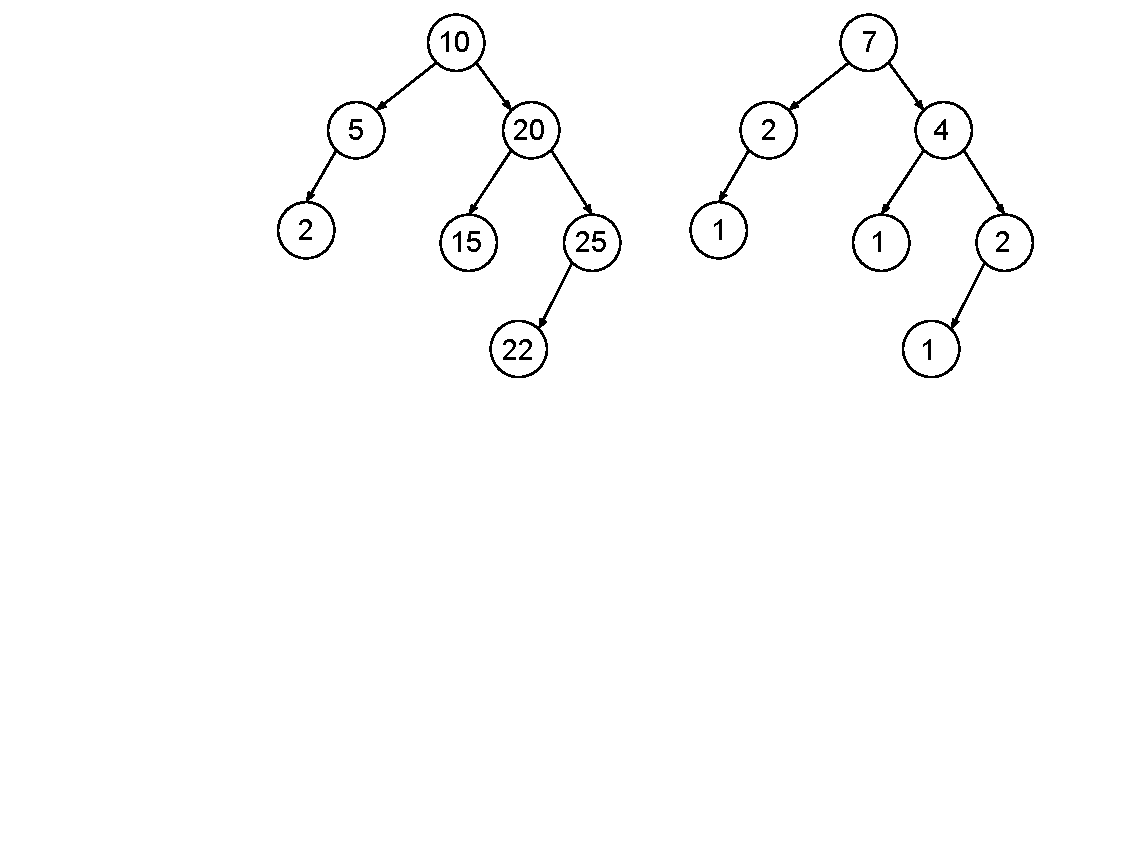
\includegraphics[width=9cm]{images/tree1}

	\vspace{-100px}

	\relscale{0.8}
	Фигура 1. Примерно дърво и същото дърво, стойностите на чиито възли са заместени с размера на съответното им поддърво.
	\end{flushleft}


	\item Стойността на всеки възел \texttt{V} в дадено двоично дърво от числа да се замени с броя на всички елементи на поддървото, на което \texttt{V} е корен. Вж. фигура 1. При операцията всеки от възлите да бъде посетен най-много веднъж.


	\begin{flushleft}
	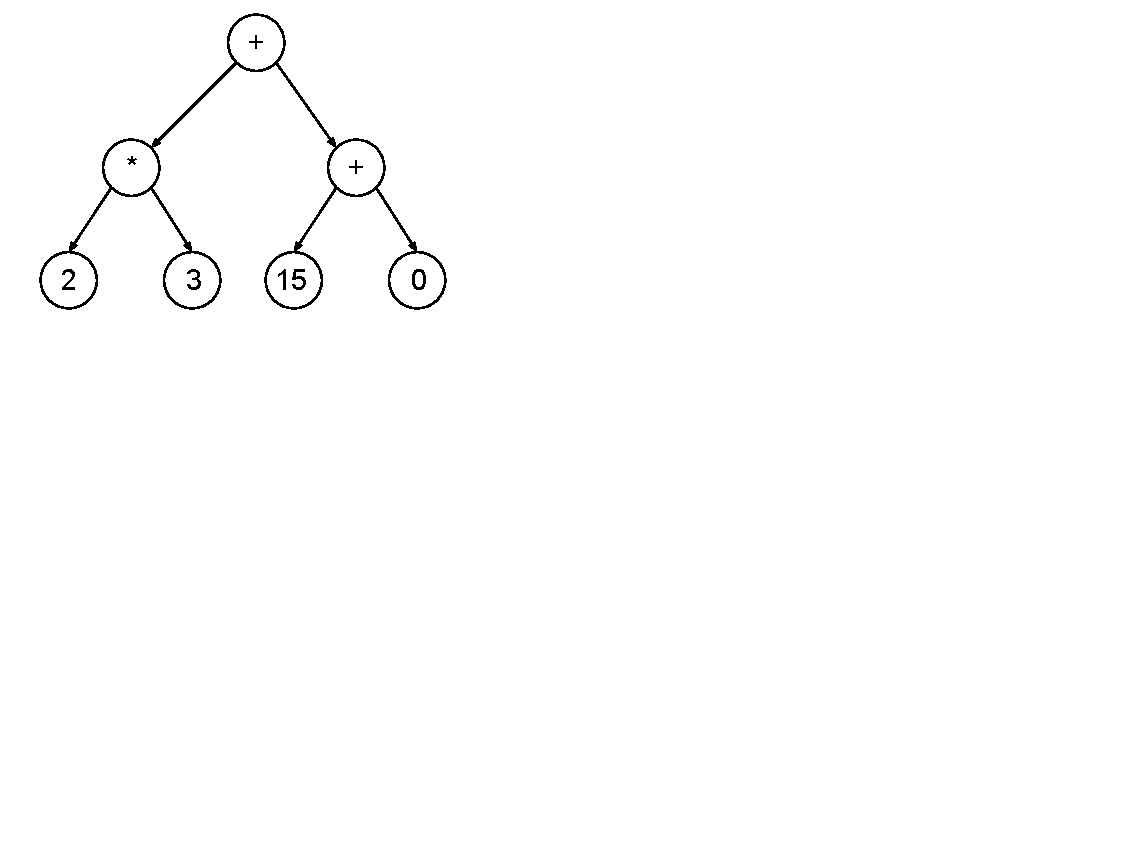
\includegraphics[width=9cm]{images/tree2}

	\vspace{-100px}

	\relscale{0.8}
	Фигура 2. Примерно дърво с аритметичен израз.
	\end{flushleft}


	\item Нека е дадено двоично дърво с елементи от тип \texttt{char}, за което е изпълнено, че:

	\begin{itemize}
		\item Дървото е непразно
		\item Всеки от възлите му има точно 2 или 0 наследника
		\item Елементите с 2 наследника съдържат един от символите $+$, $-$, $*$ и $/$
		\item Елементите с 0 наследника съдържат цифра
	\end{itemize}

	Да се дефинира функция, която връща стойността на аритметичния израз, съответен на дървото. Например, стойността на израза, съответен на дървото от фигура 2, е 21.

	б) Функцията да генерира \texttt{assertion failure}, ако дървото не отговаря на някое от описаните условия.





\end{enumerate}






\end{document}

